\documentclass[11pt,a4paper]{article}
\usepackage[margin=27mm]{geometry}
\usepackage[T1]{fontenc}
\usepackage{lmodern,microtype}
\usepackage{amsmath,amssymb,amsthm,mathtools,bm}
\usepackage{graphicx,booktabs,array}
\usepackage[dvipsnames]{xcolor}
\usepackage[colorlinks=true,linkcolor=MidnightBlue,citecolor=MidnightBlue,urlcolor=MidnightBlue]{hyperref}
\usepackage{enumitem,needspace}
\setlist{nosep}
\setlength{\parskip}{4pt}
\setlength{\parindent}{0pt}
\newtheorem{theorem}{Theorem}[section]
\newtheorem{lemma}[theorem]{Lemma}
\newtheorem{proposition}[theorem]{Proposition}
\newtheorem{corollary}[theorem]{Corollary}
\newtheorem*{theoremA}{Theorem A}
\newtheorem*{theoremB}{Theorem B}
\newtheorem*{theoremC}{Theorem C}
\theoremstyle{remark}
\newtheorem{remark}[theorem]{Remark}
\newcommand{\R}{\mathbb R}
\newcommand{\C}{\mathbb C}
\newcommand{\E}{\mathbb E}
\newcommand{\HH}{\mathcal H}
\newcommand{\dd}{\,\mathrm d}
\newcommand{\norm}[1]{\left\lVert#1\right\rVert}
\newcommand{\abs}[1]{\left|#1\right|}
\newcommand{\esssup}{\operatorname*{ess\,sup}}
\newcommand{\diag}{\operatorname{diag}}
\newcommand{\im}{\operatorname{Im}}
\newcommand{\re}{\operatorname{Re}}
\newcommand{\Mult}{\mathcal M}
\title{\textbf{Additive-noise rigidity, a sharp growth threshold and an exact nonlinear-mixture boundary for Gaussian kernel spaces}}
\author{Anonymous\\[3pt]{\small DOI \href{https://doi.org/10.5281/zenodo.24550034}{10.5281/zenodo.24550034}}}
\date{25 November 2026}
\begin{document}
\maketitle
\begin{abstract}
Kernel methods for random dynamical systems often assume that the
transition operator $Tf(x)=\E[f(X')\mid X=x]$ maps the reproducing kernel
Hilbert space (RKHS) of a Gaussian kernel boundedly into itself or into
another Gaussian RKHS. An earlier Evidence Press release proved that, for
transitions $X'=F(x)+Z$, this forces $F$ to be affine when the
characteristic function of the noise $Z$ has a Gaussian lower bound. It
asked whether that hypothesis can be removed, and whether any
state-dependent non-Gaussian transition can be admissible. We prove three
results. (A) For every probability law of $Z$, boundedness between global
Gaussian RKHSs forces $F$ to be injective and affine, and the operator
norm has an exact formula. The noise enters only through a deterministic
composition out of the stationary space with spectral measure
$|\varphi_Z|^2\mu_P$. (B) More generally, composition from any stationary
source whose spectral measure dominates Lebesgue measure near zero into
a Hilbert space of entire
functions forces an affine map whenever the logarithm of the target's
evaluation norm has zero exponential type in the imaginary direction. For
every positive type there is a target of that type admitting a bounded
nonlinear example, so the zero-type condition cannot be relaxed. (C) A finite state-dependent mixture of Gaussian
branches with a common linear part and fixed, possibly different,
covariances is bounded exactly when each mixing probability extends to an
entire function within an explicit quadratic growth budget. Nonlinear
conditional means are therefore admissible. In a scalar example a
Gaussian-bump gate $e^{-\alpha x^2}$ is admissible exactly when
$\alpha\le 8q/(1+4q)$, where $q$ is the branch variance; a probit gate
$\Phi(\beta x)$ is admissible exactly when $\beta^2\le16q/(1+4q)$; and a
logistic gate is never admissible. The Gram-matrix argument behind (C)
also gives a several-variable no-cancellation theorem for sums of
weighted composition operators on Fock spaces with a common invertible
linear part. The one-variable case of that statement was obtained
concurrently, in greater generality, by two other groups.
\end{abstract}

\section{Introduction}\label{sec:intro}

This section states the problem, explains why it matters, summarises
what was known, and lists what is new and how the paper is organised.

\paragraph{The problem.}
A Markov transition moves a state $x$ to a random state $X'$. Its
transition operator (stochastic Koopman operator) averages a test
function over one step:
\[
 Tf(x)=\E[f(X')\mid X=x].
\]
Kernel methods for learning such dynamics, such as kernel extended
dynamic mode decomposition (kernel EDMD), work with test functions from
a reproducing kernel Hilbert space (RKHS). The most common choice is the
Gaussian kernel
\[
 k_P(x,y)=\exp[-(x-y)^\top P^{-1}(x-y)],
\]
whose positive definite width matrix $P$ is chosen by the user. We write
$\HH_P(\R^m)$ for its RKHS of functions on all of $\R^m$. ``Global'' in
this paper means that norms are taken over the whole space, not over a
compact subset. The question is: \emph{for which transitions is $T$ a
bounded operator from one Gaussian RKHS into another?}

\paragraph{Why it matters.}
Some error analyses of kernel approximations of Koopman operators assume
that the RKHS is invariant under $T$; Philipp et al.\ derive full
approximation bounds under this additional hypothesis \cite{Philipp2024}.
Before such a bound can be applied to a model, one must know whether the
hypothesis can hold for it at all.

\paragraph{What was known.}
For linear stochastic differential equations, Philipp et al.\
\cite{Philipp2025} gave a sufficient condition for invariance of a
Gaussian RKHS. An earlier Evidence Press release \cite{Evidence2026}
found the exact condition and proved two rigidity statements. First, a
transition with Gaussian conditional laws $N(F(x),Q(x))$ is bounded
between Gaussian RKHSs only if $Q$ is constant and $F$ is affine. Second,
a transition $X'=F(x)+Z$ with a fixed noise variable $Z$ forces $F$ to be
affine, provided the characteristic function $\varphi$ of $Z$ satisfies
a Gaussian lower bound $|\varphi(\xi)|\ge ce^{-\xi^\top C\xi}$. That
release listed as open projects (i) whether any state-dependent
non-Gaussian transition can be bounded, and (ii) whether the lower bound
on $\varphi$ can be removed, for example for noise whose characteristic
function vanishes on an open set.

The deterministic case $Z=0$ belongs to the theory of composition
operators. Ikeda, Ishikawa and Sawano \cite{Ikeda2022} proved that
bounded composition operators on stationary RKHSs with analytic kernels
come from affine maps, under spectral hypotheses; their argument
continues an arbitrary map analytically through a Hilbert-space-valued
feature map, and we use a variant of that device. Ishikawa
\cite{Ishikawa2026} proved broad rigidity for weighted self-composition
on holomorphic function spaces. Lebedev \cite{Lebedev2012} showed that a
continuous map preserving the class of square-integrable bandlimited
functions is affine, and Hai, Huy and Tien \cite{HaiHuyTien2026} treat
weighted composition operators with entire symbols between Paley--Wiener
spaces of different bandwidths. On Fock spaces, bounded weighted
composition operators are classical \cite{TienKhoiFock2019,TienKhoi2020},
and the absence of cancellation in a difference of two of them is known
\cite[Theorem~1.4]{TienKhoi2019}.

\paragraph{What is new.}
We answer both open questions. Precise statements are in the sections
indicated.

\begin{theoremA}[Section~\ref{sec:main}]
For every probability law of the additive noise $Z$, the operator
$Tf(x)=\E f(F(x)+Z)$ maps $\HH_P(\R^m)$ boundedly into $\HH_R(\R^d)$ if
and only if $F(x)=Ax+b$ with $A$ of full column rank and a spectral
domination condition holds. The operator norm is then given exactly by
\eqref{eq:norm}.
\end{theoremA}

\begin{theoremB}[Section~\ref{sec:general}]
Let the source be any stationary RKHS whose spectral measure dominates a
multiple of Lebesgue measure near zero, and let the target be a Hilbert
space of entire functions. If $\log\norm{\operatorname{ev}_{x+iy}}$ grows
more slowly than $e^{\varepsilon|y|}$ for every $\varepsilon>0$, every
bounded operator of the form above has affine $F$. Conversely, for every
$c>0$ there are a bandlimited source and a stationary target with
$\log\norm{\operatorname{ev}_{x+iy}}\asymp e^{c|y|}$ that admit a
bounded composition with a nonlinear map.
\end{theoremB}

\begin{theoremC}[Section~\ref{sec:mixtures}]
A finite mixture $\sum_jp_j(x)\,N(Mx+b_j,Q_j)$, with pairwise
distinct pairs $(Q_j,b_j)$ and Borel probabilities $p_j$, is bounded from $\HH_P$ into $\HH_R$ if and only if $M$ has full
column rank and each $p_j$ extends to an entire function with
$|p_j(x+iy)|\le Ce^{2y^\top D_jy}$, where
$D_j=R^{-1}-M^\top(P+4Q_j)^{-1}M$.
\end{theoremC}

Theorem A settles project (ii) completely. Theorem C answers project (i)
in the affirmative and classifies a natural family: Gaussian-branch
mixtures can have nonlinear conditional means and still act boundedly,
but only with gates whose complex extensions grow at most like a
prescribed Gaussian. Section~\ref{sec:example} turns this into
statements about common gating functions. Theorem B identifies the sharp
target growth at which the affine rigidity of Theorem A stops.

\paragraph{What is not new.}
The norm formula in Theorem A follows from kernel domination and
Bochner's theorem. The multiplier criterion (Lemma~\ref{lem:multiplier})
is the Gaussian form of a classical Fock-space criterion. The smoothing
spectrum in Appendix~\ref{app:spectrum} is a classical Gaussian
integral-operator calculation. The noise in Theorem A is formal at the
operator level: Remark~\ref{rem:reduction} reduces it to deterministic
composition, so the new content of Theorems A and B is a cross-space
composition rigidity theorem with no regularity assumed on $F$ and a
sharp growth condition on the target. In Fock-space language,
Theorem~\ref{thm:mixture} is a no-cancellation statement for finite sums
of weighted composition operators with a common linear part. For one
complex variable that statement, and much more, was obtained
independently and at the same time by Cho, Choe, Koo and Tien
\cite{CCKT2026} and by Lin, Lu, Yang and Zu \cite{LLYZ2026}. Cho et al.\
note that the several-variable case is open; Corollary~\ref{cor:fock}
settles the case of a common invertible linear part. The
different-covariance classification (Theorem~\ref{thm:unequal})
involves distinct Gaussian integral operators rather than weighted
composition operators, and we did not find it in that literature.

\paragraph{Scope.}
All statements concern global RKHS norms. They do not rule out nonlinear
prediction from finite data, bounded operators on other spaces, or error
bounds in weaker norms. Recent stochastic kernel-EDMD error bounds, for
instance, use Sobolev spaces on bounded domains and Mat\'ern or Wendland
kernels, and include nonlinear examples \cite{Hertel2026}.

\paragraph{Roadmap.}
Section~\ref{sec:main} sets up notation and proves Theorem A.
Section~\ref{sec:general} proves Theorem B and its sharpness example.
Section~\ref{sec:zeros} works out noise whose characteristic function
vanishes on an open set. Section~\ref{sec:mixtures} proves Theorem C,
first for a common covariance and then for different covariances, and
gives the Fock-space form. Section~\ref{sec:example} gives exact
thresholds for scalar examples and for probit and logistic gates.
Section~\ref{sec:verification} records the computational checks and the
remaining open cases. Appendix~\ref{app:spectrum} computes the singular
values of the scalar smoothing-and-gating operator.

\paragraph{Notation.}
Throughout, $P,R,E,S\succ0$ are real symmetric positive definite width
matrices; $\HH_P(\R^m)$ is the RKHS of $k_P$; $\mu_P$ is its spectral
probability measure \eqref{eq:spectral}; $Z$ is a noise variable with
characteristic function $\varphi(\xi)=\E e^{i\xi\cdot Z}$; $Q\succeq0$
is a Gaussian covariance; and $\operatorname{ev}_z$ is evaluation at a
complex point $z=x+iy$ with $x,y$ real. Inequalities $\preceq$ between
symmetric matrices are in the positive semidefinite order.

\section{Gaussian spaces and arbitrary additive noise}\label{sec:main}

This section recalls the spectral description of Gaussian RKHSs, states
and proves Theorem A, and shows that the noise can be removed at the
operator level.

For a real symmetric positive definite $m\times m$ matrix $P$, write
$\HH_P(\R^m)$ for the complex RKHS of
$k_P(u,v)=\exp[-(u-v)^\top P^{-1}(u-v)]$. Real RKHSs may be complexified
without changing boundedness. The spectral probability measure $\mu_P$
has density
\begin{equation}\label{eq:spectral}
 \rho_P(\xi)=\frac{\sqrt{\det P}}{2^m\pi^{m/2}}
                  e^{-\xi^\top P\xi/4},
 \qquad
 k_P(u,v)=\int e^{i\xi\cdot(u-v)}\dd\mu_P(\xi).
\end{equation}
Every $f\in\HH_P$ has a unique representation
\begin{equation}\label{eq:feature}
 f(u)=U_Pg(u):=\int g(\xi)e^{i\xi\cdot u}\dd\mu_P(\xi),
 \qquad \norm{f}_P=\norm{g}_{L^2(\mu_P)}.
\end{equation}
Uniqueness follows from uniqueness of Fourier transforms of finite
measures. Cauchy--Schwarz shows that $g\rho_P\in L^1$, hence
$\HH_P\subset C_0(\R^m)$. The same representation gives an entire
extension and the exact evaluation norm
\begin{equation}\label{eq:evaluation}
 \norm{\operatorname{ev}_{x+iy}}_{\HH_P^*}
       =e^{2y^\top P^{-1}y}.
\end{equation}

Let $Z$ have any probability law on $\R^m$ and let $F:\R^d\to\R^m$ be a
Borel map. Define
\begin{equation}\label{eq:additive}
 Tf(x)=\E f(F(x)+Z).
\end{equation}
The expectation exists because Gaussian RKHS functions are bounded. The
same law of $Z$ is used at every state.

\Needspace{8\baselineskip}
\begin{theorem}[Arbitrary additive noise]\label{thm:additive}
Let $P\succ0$ and $R\succ0$ have sizes $m$ and $d$, respectively.
The following are equivalent.
\begin{enumerate}
\item $T$ maps every element of $\HH_P(\R^m)$ into $\HH_R(\R^d)$.
\item $T:\HH_P\to\HH_R$ is bounded.
\item $F(x)=Ax+b$, where $A\in\R^{m\times d}$ has full column rank,
and, for some finite $C$,
\begin{equation}\label{eq:measurecondition}
 \nu:=(A^\top)_\#\bigl(|\varphi|^2\mu_P\bigr)\le C\mu_R .
\end{equation}
\end{enumerate}
When these conditions hold,
\begin{equation}\label{eq:norm}
 \norm{T}^2=\esssup_{\eta}\frac{\dd\nu}{\dd\mu_R}(\eta).
\end{equation}
For square invertible $A$, this becomes
\begin{equation}\label{eq:squarenorm}
 \norm{T}^2=
 \frac{1}{|\det A|}\sqrt{\frac{\det P}{\det R}}\,
 \esssup_{\xi\in\R^m}
 |\varphi(\xi)|^2
 \exp\!\left[\frac{\xi^\top(ARA^\top-P)\xi}{4}\right].
\end{equation}
\end{theorem}

The theorem imposes no moment, density, infinite-divisibility, tail or
nonvanishing condition on $Z$. In particular, it includes noise whose
characteristic function vanishes on open sets (Section~\ref{sec:zeros}).

\begin{remark}[Reduction to deterministic composition]\label{rem:reduction}
Write $S_Zf(u)=\E f(u+Z)$. In the coordinates \eqref{eq:feature},
$S_Z$ multiplies the coefficient $g$ by $\varphi$. Let
$\HH_{\nu_0}$ be the stationary RKHS with spectral measure
$\nu_0=|\varphi|^2\mu_P$, whose elements are
$\int h(\xi)e^{i\xi\cdot u}\dd\nu_0(\xi)$ with norm
$\norm{h}_{L^2(\nu_0)}$. Then $S_ZU_Pg$ has coefficient
$h=g/\overline\varphi$ on $\{\varphi\ne0\}$, so
$\norm{S_ZU_Pg}^2=\int_{\{\varphi\ne0\}}|g|^2\dd\mu_P$. Thus $S_Z$ is a
partial isometry of $\HH_P$ onto $\HH_{\nu_0}$, and $T=C_F\circ S_Z$,
where $C_Ff=f\circ F$. Consequently $T:\HH_P\to\HH_R$ is bounded if and
only if $C_F:\HH_{\nu_0}\to\HH_R$ is bounded, with the same norm. Since
$|\varphi|\ge1/2$ near zero, $\nu_0$ dominates a multiple of Lebesgue
measure on a ball. The rigidity half of Theorem~\ref{thm:additive} is
therefore the case $Z=0$ of Theorem~\ref{thm:general}, applied to the
source $\HH_{\nu_0}$. We give the direct proof below because it also
yields the exact norm.
\end{remark}

\subsection{Two lemmas: local characters and zero-type growth}\label{sec:characters}

The proof has two analytic steps. The first continues the map $F$ to an
entire map from information about a local family of characters; the
second shows that slow growth of the imaginary part of that entire map
forces it to be affine. The first step adapts the holomorphic
feature-map and multiplication-map device of Ikeda, Ishikawa and Sawano
\cite[Theorem~4 and Proposition~12]{Ikeda2022}. It uses
Hilbert-space-valued holomorphy and never evaluates an arbitrary $L^2$
representative at a single frequency.

\begin{lemma}[Continuation of local characters]\label{lem:characters}
Let $B_r$ be the open ball of radius $r$ about zero in $\R^m$.
Suppose $W:\C^d\to L^2(B_r)$ is holomorphic and, for every real $x$,
\[
 W(x)(\xi)=e^{i\xi\cdot F(x)}
 \quad\text{for almost every }\xi\in B_r.
\]
Then $F$ has an entire extension $H:\C^d\to\C^m$ and
\[
 W(z)(\xi)=e^{i\xi\cdot H(z)}
 \quad\text{for almost every }\xi\in B_{r/4}.
\]
No regularity of $F$ is assumed.
\end{lemma}

\begin{proof}
The map $w\mapsto w(\xi)w(-\xi)$ is continuous quadratic from
$L^2(B_r)$ to $L^1(B_r)$. The identity theorem therefore continues
the real-state identity to
\begin{equation}\label{eq:inverse}
 W(z)(\xi)W(z)(-\xi)=1
 \quad\text{in }L^1(B_r),\qquad z\in\C^d.
\end{equation}
Likewise,
\begin{equation}\label{eq:character}
 W(z)(\xi+\eta)=W(z)(\xi)W(z)(\eta)
 \quad\text{in }L^2(B_{r/2}\times B_{r/2}).
\end{equation}
Indeed, addition pullback is bounded because
\[
 \int_{B_{r/2}\times B_{r/2}}|w(\xi+\eta)|^2\dd\xi\dd\eta
 \le |B_{r/2}|\norm{w}_{L^2(B_r)}^2 ,
\]
and $w\mapsto w\otimes w$ is continuous quadratic into the product
$L^2$ space. For either identity, apply continuous linear functionals
and the one-variable identity theorem successively in the $d$
coordinates. Agreement on $\R^d$ implies agreement on $\C^d$.

Fix $z$ and write $w=W(z)$. Equation \eqref{eq:inverse} makes $w$
nonzero almost everywhere. Choose $\psi\in C_c^\infty(B_{r/4})$ with
$c=\int w(\eta)\psi(\eta)\dd\eta\ne0$. On $B_{r/4}$ set
\[
 h(\xi)=c^{-1}\int w(\xi+\eta)\psi(\eta)\dd\eta .
\]
This function is smooth, and \eqref{eq:character} says that it equals
$w$ almost everywhere. The identities for $w$ pass to $h$ on the
smaller ball: the exceptional set for $h(\xi+\eta)$ still has product
measure zero, by the addition-pullback estimate. Continuity then gives
$h(\xi+\eta)=h(\xi)h(\eta)$ whenever all three arguments lie in the
smaller ball, as well as $h(\xi)h(-\xi)=1$. Thus $h(0)=1$.
Differentiation at $\eta=0$ gives
$\partial_jh(\xi)=a_jh(\xi)$, where $a_j=\partial_jh(0)$.
It follows that $h(\xi)=e^{a\cdot\xi}$.

The exponent varies holomorphically with $z$. Around any fixed $z_0$
choose the preceding $\psi$ so that its denominator stays nonzero.
Integration by parts gives
\begin{equation}\label{eq:exponent}
 a_j(z)=-
 \frac{\int W(z)(\eta)\,\partial_j\psi(\eta)\dd\eta}
      {\int W(z)(\eta)\,\psi(\eta)\dd\eta}.
\end{equation}
Both integrals are continuous linear functionals on $L^2(B_r)$.
These local holomorphic formulas agree on overlaps, since an
exponential character on a real open ball has a unique exponent.
Consequently $a$ is entire. Set $H=a/i$. Uniqueness at each real
state gives $H(x)=F(x)$.
\end{proof}

\begin{lemma}[Zero-type imaginary growth forces affineness]\label{lem:growth}
Let $H:\C^d\to\C^m$ be entire and real-valued on $\R^d$. Suppose that
for every $\varepsilon>0$ there is $C_\varepsilon<\infty$ with
\begin{equation}\label{eq:zerotype}
 |\im H(x+iy)|\le C_\varepsilon e^{\varepsilon|y|}\qquad(x,y\in\R^d).
\end{equation}
Then $H(z)=Az+b$ with real $A$ and $b$. In particular this holds if
$|\im H(x+iy)|\le C(1+|y|^s)$ for some $C$ and $s\ge0$.
\end{lemma}

\begin{proof}
Fix a component $H_j$, a real base point $x_0$ and a real direction
$v\ne0$, and put $g(t)=H_j(x_0+tv)$ for $t\in\C$. Then $g$ is entire,
real on $\R$, and $u=\im g$ is harmonic with
$|u(s+i\tau)|\le C_\varepsilon e^{\varepsilon|v||\tau|}$ for all
real $s,\tau$ and every $\varepsilon>0$.

\emph{Step 1: $g'$ has a uniform horizontal bound.}
By the Cauchy--Riemann equations $|g'|=|\nabla u|$. The gradient
estimate for harmonic functions on the unit disc about $t$ gives
$|\nabla u(t)|\le 2\sqrt2\sup_{|t'-t|<1}|u(t')|$. Hence
\[
 |g'(t)|\le K_\varepsilon e^{\varepsilon|v||\im t|},\qquad
 K_\varepsilon=2\sqrt2\,C_\varepsilon e^{\varepsilon|v|},
\]
for all $t\in\C$. In particular $g'$ is bounded on $\R$, say by $K$.

\emph{Step 2: $g'$ is constant.}
Fix $\varepsilon>0$ and put $\delta=\varepsilon|v|$ and
$G(t)=g'(t)e^{2i\delta t}$. On the closed upper half-plane
$|G(t)|\le K_\varepsilon e^{-\delta\im t}\le K_\varepsilon$, and
$|G|\le K$ on $\R$. For $\theta>0$ the function $G(t)/(1-i\theta t)$
is holomorphic on the upper half-plane, continuous up to its boundary,
bounded there by $K$ on $\R$, and tends to zero at infinity because
$|1-i\theta t|\ge1+\theta\im t$ and $|1-i\theta t|\to\infty$. The
maximum principle bounds it by $K$; letting $\theta\to0$ gives
$|G|\le K$, that is, $|g'(t)|\le Ke^{2\delta\im t}$ for $\im t\ge0$.
The same argument with $e^{-2i\delta t}$ applies in the lower
half-plane. Since $\varepsilon>0$ was arbitrary, $|g'|\le K$ on $\C$,
and Liouville's theorem makes $g'$ constant.

\emph{Step 3: conclusion.}
Thus $g(t)=g(0)+tg'(0)$, with real coefficients because $g$ is real on
$\R$. Taking $x_0=0$, every real line through the origin is mapped
affinely: $H(tv)=H(0)+t\,DH(0)v$ for real $t$ and $v$. This determines
$H$ on $\R^d$ as the affine map $x\mapsto H(0)+DH(0)x$, and then on
$\C^d$ by uniqueness of entire extensions. Polynomial growth
$C(1+|y|^s)$ is bounded by $C_\varepsilon e^{\varepsilon|y|}$ for every
$\varepsilon>0$.
\end{proof}

\subsection{Proof of Theorem \ref{thm:additive}}

The proof represents evaluation of $Tf$ at a complex point by a
holomorphic family of source coefficients, divides out the noise only
near frequency zero, and then applies the two lemmas.

\begin{proof}
First, inclusion implies boundedness by the closed graph theorem.
Convergence in either Gaussian RKHS implies uniform convergence on
the real domain, since $k_P(x,x)=k_R(x,x)=1$. Source convergence
$f_n\to f$ therefore implies $Tf_n\to Tf$ uniformly. If also
$Tf_n\to h$ in $\HH_R$, the same uniform limit is $h=Tf$.

Assume now that $T$ is bounded. For each complex $z$, consider the
complex-linear functional
$\operatorname{ev}_z\circ T\circ U_P$ on $L^2(\mu_P)$.
Using the complex-bilinear pairing $(g,V)\mapsto\int gV\dd\mu_P$,
write it uniquely as
\[
 g\longmapsto\int g(\xi)V_z(\xi)\dd\mu_P(\xi).
\]
We call $V_z$ the source representer of $\operatorname{ev}_z\circ T$.
The map $z\mapsto V_z$ is holomorphic into $L^2(\mu_P)$ and
\begin{equation}\label{eq:Vbound}
 \norm{V_z}_{L^2(\mu_P)}
 \le \norm{T}e^{2(\im z)^\top R^{-1}(\im z)}.
\end{equation}
Holomorphy follows either by transposing the holomorphic evaluation
map, or from weak holomorphy and the locally uniform bound in
\eqref{eq:Vbound}. Fubini's theorem in \eqref{eq:feature} gives,
at real states,
\[
 V_x(\xi)=\varphi(\xi)e^{i\xi\cdot F(x)}.
\]
There is no conjugation ambiguity in this bilinear convention.

Every characteristic function is continuous and equals one at zero.
Choose $r>0$ so that $|\varphi|\ge1/2$ on $B_r$. Since $\rho_P$ is
bounded below there, restriction followed by division by $\varphi$
is a bounded map $L^2(\mu_P)\to L^2(B_r)$.
Apply Lemma \ref{lem:characters} to $W(z)=V_z/\varphi$ on this ball.
It supplies an entire extension $H$ of $F$ and
\begin{equation}\label{eq:capupper}
 \int_{B_{r/4}}e^{-2\xi\cdot\im H(z)}\dd\xi
 \le C_1\norm{V_z}^2_{L^2(\mu_P)}
 \le C_1\norm T^2e^{4(\im z)^\top R^{-1}(\im z)}.
\end{equation}
If $v=\im H(z)\ne0$, the cap
$\{\xi\in B_{r/4}:\xi\cdot v\le-r|v|/8\}$ has a fixed positive
volume $c_1$ independent of the direction of $v$. The integral on the
left is therefore at least $c_1e^{r|v|/4}$.
Taking logarithms proves
$|\im H(x+iy)|\le C_2+C_3|y|^2$.
Lemma \ref{lem:growth} makes $F(x)=Ax+b$.

If $Av=0$ for a nonzero real $v$, choose
$f(u)=k_P(u,0)>0$. Then $Tf(x+tv)=Tf(x)>0$ for all real $t$,
contradicting $\HH_R\subset C_0$. Hence $A$ has full column rank.

For affine $F$, the Gram kernel of the source evaluation
representers is
\begin{equation}\label{eq:gramstationary}
 K_T(x,y)=\int e^{i\xi\cdot A(x-y)}|\varphi(\xi)|^2\dd\mu_P(\xi)
         =\int e^{i\eta\cdot(x-y)}\dd\nu(\eta).
\end{equation}
The usual kernel-domination argument is short: on the dense span
of output kernel sections, define
$\sum c_jk_R(\,\cdot\,,x_j)\mapsto\sum c_jh_{x_j}$,
where $h_{x_j}$ is the source representer. This map has squared
norm at most $C$ exactly when $Ck_R-K_T$ is positive definite.
Its adjoint then equals $T$ on every real evaluation.
By Bochner's theorem and uniqueness of Fourier transforms of finite
measures, this kernel condition is equivalent to
$C\mu_R-\nu\ge0$. This proves the converse and \eqref{eq:norm}.
A linear change of variables yields \eqref{eq:squarenorm}.
\end{proof}

If $A$ is rectangular and has full column rank, the linear coarea
formula gives the density
\begin{equation}\label{eq:coarea}
 \frac{\dd\nu}{\dd\eta}(\eta)=
 \frac{1}{\sqrt{\det(A^\top A)}}
 \int_{A^\top\xi=\eta}|\varphi(\xi)|^2\rho_P(\xi)
                   \dd\mathcal H^{m-d}(\xi),
\end{equation}
where $\mathcal H^{m-d}$ is Euclidean Hausdorff measure on the fibre.

\begin{corollary}[Essential norm]\label{cor:essential}
Every bounded operator in Theorem \ref{thm:additive} satisfies
$\norm{T}_{\rm ess}=\norm{T}>0$ and is noncompact.
\end{corollary}

\begin{proof}
For a nonzero $v\in\R^d$, source translation by $tAv$ intertwines
with output translation by $tv$. Both translations are unitary
in their respective Gaussian RKHSs. For any fixed source function,
translations by $nAv$ tend weakly to zero: in spectral coordinates
this is the Riemann--Lebesgue lemma applied to a product of two
$L^2(\mu_P)$ coefficients. A compact operator sends this sequence
to zero in norm, whereas the norms of its $T$-images are constant.
Thus $\norm{T-K}\ge\norm{Tf}$ for every compact $K$ and every unit
source $f$. Taking the supremum proves the assertion. Positivity
of the Gaussian probe in the preceding proof ensures $T\ne0$.
\end{proof}

\section{The sharp target-growth threshold}\label{sec:general}

This section isolates what the rigidity argument needs from the source
and the target, and shows that the condition on the target cannot be
weakened in the exponential-type scale.

A finite positive measure $\mu$ on $\R^m$ defines the stationary RKHS
$\HH_\mu$ of functions $\int g(\xi)e^{i\xi\cdot u}\dd\mu(\xi)$,
$g\in L^2(\mu)$, normed by $\norm{g}_{L^2(\mu)}$. For a Hilbert space
$\mathcal K$ of entire functions on $\C^d$ with continuous evaluations,
we measure growth in the imaginary direction by
\[
 \Lambda_{\mathcal K}(y)=\sup_{x\in\R^d}
 \log\norm{\operatorname{ev}_{x+iy}}_{\mathcal K^*}.
\]
For $\HH_R$ this is the quadratic $2y^\top R^{-1}y$ by
\eqref{eq:evaluation}. For a Paley--Wiener space it is linear in $|y|$.

\begin{theorem}[Zero-type targets]\label{thm:general}
Let $\mu$ be a finite positive measure on $\R^m$ such that
$\mu\ge c\,1_{B_r}\dd\xi$ for some $c,r>0$. Let $\mathcal K$ be a
Hilbert space of entire functions on $\C^d$ with continuous evaluations,
and suppose that for every $\varepsilon>0$ there is $C_\varepsilon$
with
\begin{equation}\label{eq:zerotypetarget}
 \Lambda_{\mathcal K}(y)\le C_\varepsilon e^{\varepsilon|y|}
 \qquad(y\in\R^d).
\end{equation}
If \eqref{eq:additive}, for any probability law of $Z$, defines a
bounded map $\HH_\mu\to\mathcal K$, then $F$ is affine. If in addition
$\mathcal K\subset C_0(\R^d)$, its linear part has full column rank.
\end{theorem}

\begin{proof}
The feature map $g\mapsto\int g(\xi)e^{i\xi\cdot u}\dd\mu(\xi)$
is an isometry onto $\HH_\mu$; uniqueness follows from Fourier
uniqueness. Its functions are bounded because $\mu$ is finite.
Repeat the bilinear-representer construction in the preceding proof.
On a smaller ball, $\varphi$ is bounded away from zero and $\mu$
dominates Lebesgue measure, so Lemma \ref{lem:characters} applies.
The cap estimate now gives
\[
 c_1e^{r|\im H(z)|/4}\le C_1\norm{T}^2
 \norm{\operatorname{ev}_z}^2_{\mathcal K^*},
\]
hence $|\im H(x+iy)|\le C'+(8/r)\Lambda_{\mathcal K}(y)$, which
satisfies \eqref{eq:zerotype}. Lemma \ref{lem:growth} gives
affineness.

For the rank assertion, the real-state source representer has
squared norm $\int|\varphi|^2\dd\mu>0$, since the integrand is
bounded below near zero. Thus some source $f$ has $Tf(x_0)\ne0$.
A null direction of the affine linear part makes this output
constant and nonzero along a line, contradicting $C_0$.
\end{proof}

The source need not be analytic. A Mat\'ern spectral density, for
example, has the required local lower bound. This says that a
Mat\'ern \emph{source} mapped boundedly into a zero-type entire
target has affine drift; it does not impose affine rigidity on
Mat\'ern self-composition. Targets with spectral densities proportional
to $e^{-a|\xi|^p}$, $p>1$, satisfy \eqref{eq:zerotypetarget}, since
$\Lambda$ then grows like $|y|^{p/(p-1)}$ by Young's inequality.
Compactly supported spectral densities give linear $\Lambda$. With
$Z=0$ and a Paley--Wiener source and target, Theorem~\ref{thm:general}
gives a single-band variant of Lebedev's theorem \cite{Lebedev2012}: a
bounded composition operator into one Paley--Wiener space comes from an
affine map, with no continuity assumed on $F$. Lebedev's theorem itself
concerns maps preserving the whole class of bandlimited functions, for
continuous maps.

\subsection{Positive type allows nonlinear maps}

The zero-type hypothesis cannot be relaxed to any positive exponential
type. The example adapts the factorial spectral weights of Ikeda et al.\
\cite[Corollary~1]{Ikeda2022}; their theorem concerns self-composition,
whereas here the source and target differ.

\begin{proposition}[A nonlinear bounded cross-space composition]\label{prop:warping}
Fix $0<a<1/2$ and $0<\varepsilon<1$. Let the source spectral
density be $(2a)^{-1}1_{[-a,a]}$, and let the target density be
\[
 \rho_\star(\eta)=
 \frac{1}{2a\kappa}\sum_{n\in\mathbb Z}
          \frac{1_{n+[-a,a]}(\eta)}{|n|!},
 \qquad \kappa=2e-1.
\]
Then $F(x)=x+\varepsilon\sin x$ is nonlinear, and
$C_Ff=f\circ F$ is bounded from the source to the target.
Its exact squared norm is
\begin{equation}\label{eq:besselnorm}
 \norm{C_F}^2=
 \kappa\esssup_{|\xi|\le a}
       \sum_{n\in\mathbb Z}|n|!\,|J_n(\varepsilon\xi)|^2<\infty,
\end{equation}
where $J_n$ is the Bessel function of the first kind.
The stationary target kernel is
\begin{equation}\label{eq:infinitekernel}
 k_\star(t)=\frac{\sin(at)}{at}\,
       \frac{e^{e^{it}}+e^{e^{-it}}-1}{2e-1},
\end{equation}
and its growth function satisfies
\begin{equation}\label{eq:typetwo}
 e^{2|y|}-\log\kappa\le2\Lambda_\star(y)\le e^{2|y|}+2a|y|.
\end{equation}
\end{proposition}

\begin{proof}
For $f(x)=(2a)^{-1}\int_{-a}^ag(\xi)e^{i\xi x}\dd\xi$,
the Jacobi--Anger expansion gives
\[
 f(F(x))=\frac1{2a}\sum_{n\in\mathbb Z}
   \int_{-a}^a g(\xi)J_n(\varepsilon\xi)e^{i(\xi+n)x}\dd\xi .
\]
The bands $n+[-a,a]$ are disjoint, so the squared target norm is
\[
 \frac \kappa{2a}\int_{-a}^a|g(\xi)|^2
       \sum_{n\in\mathbb Z}|n|!\,|J_n(\varepsilon\xi)|^2\dd\xi .
\]
This proves \eqref{eq:besselnorm}. For real $t$ the defining
Bessel series gives
$|J_n(t)|\le e^{t^2/4}(|t|/2)^{|n|}/|n|!$.
Thus the sum is bounded, uniformly on the source band, by
$e^{t^2/2}(2e^{t^2/4}-1)$.
This bound also justifies interchange of the series and integral.
Summing the target spectral Fourier series proves
\eqref{eq:infinitekernel}. Finally, the target is stationary, and at
$z=x+iy$ its squared evaluation norm is
\[
 \int e^{-2\eta y}\rho_\star(\eta)\dd\eta
 =\frac{\sinh(2ay)}{2ay}\,
   \frac{e^{e^{2y}}+e^{e^{-2y}}-1}{2e-1}.
\]
Since $1\le\sinh(s)/s\le e^{|s|}$, $1\le e^{e^{-2|y|}}\le e$ and
$\kappa\ge e$, this lies between $e^{e^{2|y|}}/\kappa$ and
$e^{2a|y|}e^{e^{2|y|}}$, which is \eqref{eq:typetwo}.
\end{proof}

\begin{corollary}[Sharpness of the zero-type condition]\label{cor:sharp}
For every $c>0$ there are a stationary source with spectral density
bounded below near zero, a stationary target $\mathcal K_c\subset
C_0(\R)$ with $\Lambda_{\mathcal K_c}(y)\le(e^{c|y|}+ac|y|)/2$, and a
nonlinear map $F_c(x)=x+(2\varepsilon/c)\sin(cx/2)$ such that $C_{F_c}$
is bounded from the source to $\mathcal K_c$. Moreover
$\Lambda_{\mathcal K_c}(y)\ge(e^{c|y|}-\log\kappa)/2$, so the type of
$\mathcal K_c$ is exactly $c$.
\end{corollary}

\begin{proof}
Put $\lambda=c/2$ and write $D_\lambda h(x)=h(\lambda x)$. Dilation
$D_\lambda$ is unitary from a stationary RKHS onto the stationary RKHS
whose spectral measure is the image under $\xi\mapsto\lambda\xi$. If
$F$ is the map of Proposition~\ref{prop:warping}, then
$F_c(x)=\lambda^{-1}F(\lambda x)$ and
$C_{F_c}=D_\lambda C_FD_{\lambda}^{-1}$, so $C_{F_c}$ is bounded
between the dilated spaces with the same norm. The dilated source has
spectral density bounded below on $[-\lambda a,\lambda a]$. Evaluation
at $iy$ in the dilated target equals evaluation at $i\lambda y$ in the
original target, and \eqref{eq:typetwo} gives the two bounds.
\end{proof}

Together, Theorem~\ref{thm:general} and Corollary~\ref{cor:sharp} show
that the zero-type condition on the target cannot be relaxed: affine
rigidity holds for every target of zero exponential type, and for every
positive type some target of that type, paired with a bandlimited
source, admits a nonlinear map. The examples use bandlimited sources;
whether a Gaussian source can be mapped nonlinearly into a target of
positive type is not settled here. Gaussian and Paley--Wiener targets lie
far inside the rigid range.

\section{Noise with spectral zeros}\label{sec:zeros}

This section applies Theorem~\ref{thm:additive} to noise that the
earlier lower-bound hypothesis excluded, and computes the resulting
norms exactly.

The noise law
\begin{equation}\label{eq:triangular}
 p_Z(z)=\frac{1-\cos z}{\pi z^2},\qquad
 p_Z(0)=\frac1{2\pi},
 \qquad
 \varphi(\xi)=(1-|\xi|)_+
\end{equation}
has a characteristic function that vanishes for $|\xi|\ge1$. Fourier
inversion of the triangular function gives the displayed nonnegative
density, whose integral is one. Theorem~\ref{thm:additive} still forces
affine drift.

On $\HH_1(\R)$, however, every nonzero affine slope $a$ is allowed
for this noise. Formula \eqref{eq:squarenorm} gives
\begin{equation}\label{eq:triangularnorm}
 \norm{T_a}^2=\frac1{|a|}
       \max_{0\le t\le1}(1-t)^2
                    e^{ct^2},\qquad c=\frac{a^2-1}{4}.
\end{equation}
This is finite for every $a\ne0$. The maximand equals $1$ at $t=0$, and
it is at most $1$ on $[0,1]$ exactly when $c\le-2\log(1-t)/t^2$ for all
$0<t<1$. Hence
\begin{equation}\label{eq:astar}
 \norm{T_a}^2=\frac1{|a|}\iff
 a^2\le a_*^2:=1+4c_*,\qquad
 c_*=\min_{0<t<1}\frac{-2\log(1-t)}{t^2},
\end{equation}
with $c_*\approx4.91081$ attained at $t\approx0.71533$ and
$a_*\approx4.54349$; for $|a|>a_*$ the norm is strictly larger. In
particular the slopes $1,2,3,4$ give the exact squared norms
$1,1/2,1/3,1/4$. Noise with a frequency cut-off can therefore admit
arbitrarily expansive affine maps, while it never admits a nonlinear
drift.

This phenomenon does not require heavy tails. Choose a nonzero
$h\in C_c^\infty(\R)$ and use the probability density proportional to
$|\mathcal F^{-1}h|^2$. It is a nonnegative Schwartz density, and its
characteristic function is the normalised autocorrelation of $h$, hence
has compact support. For a square invertible affine map, the supremum
in \eqref{eq:squarenorm} is again finite for every pair of positive
Gaussian widths. All moments of this noise law exist.

\section{Finite Gaussian mixtures}\label{sec:mixtures}

This section proves Theorem C: it classifies bounded finite mixtures of
Gaussian branches with state-dependent probabilities, first when all
branches share one covariance and then when the covariances differ.

Fix $P\succ0$, $R\succ0$, a real $m\times d$ matrix $M$,
a covariance matrix $Q\succeq0$, and pairwise distinct shifts
$b_1,\ldots,b_N\in\R^m$. Let the Borel probabilities
$p_j:\R^d\to[0,1]$ sum to one. Consider
\begin{equation}\label{eq:mixture}
 Tf(x)=\sum_{j=1}^Np_j(x)\E f(Mx+b_j+G),\qquad
                         G\sim N(0,Q).
\end{equation}
The common linear part $M$ and the finite fixed shift set are
substantive restrictions; the common covariance is removed in
Section~\ref{sec:different}.

\Needspace{15\baselineskip}
\begin{theorem}[Finite-mixture classification]\label{thm:mixture}
The operator \eqref{eq:mixture} maps $\HH_P(\R^m)$ boundedly
into $\HH_R(\R^d)$ if and only if $M$ has full column rank and
each $p_j$ extends to an entire function satisfying
\begin{equation}\label{eq:weightbound}
 B_j:=\sup_{z=x+iy}|p_j(z)|e^{-2y^\top Dy}<\infty,\qquad
 D=R^{-1}-M^\top(P+4Q)^{-1}M .
\end{equation}
These conditions imply $D\succeq0$. Every $p_j$ is constant
along each complex direction in $\ker D$; if $D=0$, all
probabilities are constant. Conversely, if $D\succeq0$ has a
positive direction and at least two branches are
available, it permits nonconstant probability weights.
\end{theorem}

The matrix $P+4Q$ appears because the norm compares two independent
copies of the Gaussian noise, whose difference has covariance $2Q$, on
top of the kernel width $P$; this is the same factor $4$ as in
\cite{Evidence2026}.

\subsection{The multiplier calculation}

The sufficiency half rests on the following Gaussian-RKHS form of the
classical Fock-space criterion for weighted composition and
multiplication operators \cite{TienKhoiFock2019,TienKhoi2020}. We
include the proof to fix the anisotropic normalisation and the equality
case.

\begin{lemma}[Gaussian multipliers]\label{lem:multiplier}
For $E,R\succ0$, multiplication $\Mult_p$ by $p$ maps $\HH_E$ boundedly
into $\HH_R$ if and only if $p$ extends to an entire function with
\[
 B(p):=\sup_{x+iy}|p(x+iy)|
                e^{-2y^\top(R^{-1}-E^{-1})y}<\infty.
\]
Moreover
\begin{equation}\label{eq:multipliernorm}
 B(p)\le\norm{\Mult_p}
       \le\sqrt{\frac{\det E}{\det R}}\,B(p).
\end{equation}
For $p(x)=e^{-(x-c)^\top\Omega(x-c)}$, with $c\in\R^d$ and $\Omega$ real
symmetric, the condition is exactly
\begin{equation}\label{eq:Gaussianweight}
 0\preceq \Omega\preceq2(R^{-1}-E^{-1}).
\end{equation}
\end{lemma}

\begin{proof}
If $\Mult_p$ is bounded, apply it to the nowhere-zero section
$e^{-x^\top E^{-1}x}$ and divide its entire output by the
nowhere-zero entire section. This gives the entire extension of
$p$. Evaluation at $z$ and \eqref{eq:evaluation} give the lower
bound in \eqref{eq:multipliernorm}.

For sufficiency, Gaussian RKHSs have the exact tube norm
\begin{equation}\label{eq:tubenorm}
 \norm{f}_P^2=
 \frac{2^d}{\pi^d\det P}
 \int_{\R^d\times\R^d}|f(x+iy)|^2
                  e^{-4y^\top P^{-1}y}\dd x\dd y .
\end{equation}
To see both the formula and its characterisation of the space,
multiply $f(z)$ by $e^{z^\top P^{-1}z}$. The resulting space has
Fock kernel $e^{2z^\top P^{-1}\overline w}$ and its Gaussian
integral norm; expanding the exponential in monomials verifies
the isometry. Alternatively, Plancherel in $x$ and a Gaussian
integral in $y$ give the same constants in \eqref{eq:tubenorm}.
Inserting the growth bound for $p$ in this norm proves the
upper bound in \eqref{eq:multipliernorm}.
For the Gaussian weight, its absolute value at $x+iy$ is
$e^{-(x-c)^\top \Omega(x-c)+y^\top \Omega y}$, proving
\eqref{eq:Gaussianweight}, including semidefinite equality.
\end{proof}

\subsection{Proof of Theorem \ref{thm:mixture}}

The proof first recovers the weights as entire functions from the
images of finitely many kernel sections, then bounds each weight by
evaluating $T$ at complex points, and finally assembles sufficiency
from Lemma~\ref{lem:multiplier}.

\begin{proof}
If $Mv=0$ for $v\ne0$, fix $x$ and take the positive kernel
section $f=k_P(\,\cdot\,,0)$. Every component expectation on
$x+tv$ is a strictly positive constant, independent of $t$.
Their convex combination is bounded below by the smallest
of these finitely many constants. This contradicts
$Tf\in C_0$. Thus $M$ has full column rank. Put
\[
 S=P+4Q,\qquad U=P+2Q,\qquad
 E=(M^\top S^{-1}M)^{-1},\qquad
 c_V=\sqrt{\det P/\det V}.
\]

\emph{Recovering the weights.}
Apply $T$ to the $N$ sections $f_i(u)=k_P(u,b_i)$.
Gaussian integration gives
\[
 Tf_i(x)=c_U\sum_jp_j(x)
   e^{-(Mx+b_j-b_i)^\top U^{-1}(Mx+b_j-b_i)}.
\]
The matrix of these coefficients at complex $z$ factors as
\begin{align}\label{eq:testmatrix}
 \Gamma(z)={}&c_Ue^{-z^\top M^\top U^{-1}Mz}
 \diag_i(e^{2z^\top M^\top U^{-1}b_i})\,G_U\,
 \diag_j(e^{-2z^\top M^\top U^{-1}b_j}),\\
 (G_U)_{ij}={}&e^{-(b_i-b_j)^\top U^{-1}(b_i-b_j)}.\notag
\end{align}
$G_U$ is strictly positive definite: its spectral density is
positive everywhere, and a nonzero finite exponential sum
cannot vanish almost everywhere. All remaining factors in
\eqref{eq:testmatrix} are nowhere zero. Thus $\Gamma(z)^{-1}$ is
entire. Since the $Tf_i$ extend to entire functions, so does
$p(z)=\Gamma(z)^{-1}(Tf_i(z))_i$. The identity $\sum_jp_j=1$
continues to all complex states.

\emph{Controlling each weight.}
Let $h_j(z)$ be the source representer of evaluation of the $j$th pure
branch at $z$. Its bilinear representative is
$e^{-\xi^\top Q\xi/2}e^{i\xi\cdot(Mz+b_j)}$.
For $z=x+iy$, direct Gaussian integration gives the Hermitian
Gram matrix
\begin{equation}\label{eq:unitarygram}
 \bigl(\langle h_i(z),h_j(z)\rangle\bigr)_{ij}
 =c_Se^{4y^\top E^{-1}y}\,\Theta_yG_S\Theta_y^*,
\end{equation}
up to the transpose associated with the inner-product convention,
where $\Theta_y$ is diagonal unitary and
$(G_S)_{ij}=e^{-(b_i-b_j)^\top S^{-1}(b_i-b_j)}$.
For example, the entry's phase is
$e^{-4i\,y^\top M^\top S^{-1}(b_i-b_j)}$ in the
linear-first convention. The eigenvalues of the fixed
$G_S$ are strictly positive.

The branch formula with the now-entire weights holds at
complex states by uniqueness of entire extension. If
$\lambda_*>0$ is the smallest eigenvalue of $G_S$,
\begin{equation}\label{eq:weightnecessity}
 c_S\lambda_*e^{4y^\top E^{-1}y}
                  \sum_j|p_j(z)|^2
 \le \norm{\operatorname{ev}_z\circ T}^2
 \le \norm{T}^2e^{4y^\top R^{-1}y}.
\end{equation}
This proves every bound in \eqref{eq:weightbound}.
In particular, complex cancellation between finitely many
branches cannot conceal excessive weight growth.

\emph{Sufficiency.}
Each pure branch $L_jf(x)=\E f(Mx+b_j+G)$ has source-representer
kernel exactly $c_Sk_E(x,y)$. Kernel domination therefore
gives $L_j:\HH_P\to\HH_E$ with squared norm $c_S$.
Lemma \ref{lem:multiplier} makes
$\Mult_{p_j}:\HH_E\to\HH_R$ bounded under
\eqref{eq:weightbound}. Their finite sum is $T$.

\emph{The boundary.}
From $\sum_jp_j(z)=1$,
$1\le(\sum_jB_j)e^{2y^\top Dy}$ for every $y$.
A negative direction of $D$ is impossible.
If $v\in\ker D$, the entire function
$t\mapsto p_j(z_0+tv)$ is bounded on $\C$, since the quadratic
form in \eqref{eq:weightbound} is unchanged. Liouville's theorem
makes it constant. Finally, if $D$ has a positive direction,
choose a nonzero $a\in\operatorname{range}D$ and a sufficiently
small $\alpha>0$ with $\alpha aa^\top\preceq2D$.
The probabilities $p_1(x)=e^{-\alpha(a^\top x)^2}$,
$p_2(x)=1-p_1(x)$, with all other probabilities zero, satisfy
the criterion and are nonconstant.
\end{proof}

\subsection{The Fock-space form}

This subsection translates the Gram argument into the language of
weighted composition operators, where it gives a several-variable
no-cancellation statement. For $\omega>0$ let $F^2_\omega(\C^d)$ be the
Fock space of entire $f$ with
$\norm{f}_\omega^2=(\omega/\pi)^d\int_{\C^d}|f(z)|^2e^{-\omega|z|^2}\dd
A(z)<\infty$. Its reproducing kernel is $K^\omega_w(z)=e^{\omega\langle
z,w\rangle}$, with $\norm{K^\omega_w}^2=e^{\omega|w|^2}$. For an entire
weight $\psi$ and an entire map $\phi$, the weighted composition
operator is $W_{\psi,\phi}f=\psi\cdot(f\circ\phi)$.

\begin{corollary}[Common linear part in several variables]\label{cor:fock}
Let $\mathcal A\in\C^{d\times d}$ be invertible, let $b_1,\dots,b_N\in\C^d$ be
pairwise distinct, let $\psi_1,\dots,\psi_N$ be entire, and let
$\omega_1,\omega_2>0$. Then $T=\sum_jW_{\psi_j,\mathcal Az+b_j}$ maps $F^2_{\omega_1}(\C^d)$
boundedly into $F^2_{\omega_2}(\C^d)$ if and only if, for every $j$,
\begin{equation}\label{eq:fockgauge}
 \sup_{z\in\C^d}|\psi_j(z)|
 \exp\Bigl(\tfrac{\omega_1}{2}|\mathcal Az+b_j|^2-\tfrac{\omega_2}{2}|z|^2\Bigr)<\infty,
\end{equation}
and this holds if and only if every summand $W_{\psi_j,\mathcal Az+b_j}$ is
bounded.
\end{corollary}

\begin{proof}
For a single operator, the dilation $f\mapsto f(\gamma\,\cdot)$ is
unitary from $F^2_{\omega_1}$ onto $F^2_{\omega_1\gamma^2}$; conjugating by
dilations reduces $W_{\psi,\phi}:F^2_{\omega_1}\to F^2_{\omega_2}$ to a weighted
composition operator on $F^2_1$ with an invertible affine symbol and
the same value of the supremum \eqref{eq:fockgauge}. Tien and Khoi
\cite[Corollary~3.10(a)]{TienKhoi2020} prove that such an operator is
bounded exactly when this supremum is finite; a summand with
$\psi_j\equiv0$ is trivially bounded. (Its finiteness also gives
the membership conditions in their class of admissible pairs: the
symbol's linear part has norm at most one by their Proposition~2.6, and
the weight lies in the Fock space because $\mathcal A$ is invertible.) Hence
\eqref{eq:fockgauge} for every $j$ is equivalent to boundedness of every
summand, which implies boundedness of $T$.

Conversely, suppose $T$ is bounded. For $f\in F^2_{\omega_1}$,
$\langle Tf,K^{\omega_2}_z\rangle_{\omega_2}=\sum_j\psi_j(z)f(\mathcal Az+b_j)$, so
$T^*K^{\omega_2}_z=\sum_j\overline{\psi_j(z)}K^{\omega_1}_{w_j}$ with
$w_j=\mathcal Az+b_j$. With $k_w=K^{\omega_1}_w/\norm{K^{\omega_1}_w}$,
\[
 \langle k_{w_j},k_{w_i}\rangle
 =\exp\bigl(-\tfrac{\omega_1}{2}|w_i-w_j|^2+i\omega_1\im\langle w_i,w_j\rangle\bigr).
\]
Writing $w_j=u+b_j$ with $u=\mathcal Az$, we have $w_i-w_j=b_i-b_j$ and
$\im\langle w_i,w_j\rangle=\im\langle u,b_j\rangle-\im\langle u,b_i\rangle
+\im\langle b_i,b_j\rangle$. So the normalised Gram matrix at $z$ equals
$\Theta G_0\Theta^*$, where $\Theta$ is diagonal unitary and $G_0$ is the
normalised Gram matrix of the kernels at the distinct points $b_j$.
These kernels are linearly independent, because point evaluations at
distinct points are independent on polynomials. Hence the smallest
eigenvalue $\lambda_0$ of $G_0$ is positive, and
\[
 \lambda_0\sum_j|\psi_j(z)|^2e^{\omega_1|\mathcal Az+b_j|^2}
 \le\norm{T^*K^{\omega_2}_z}^2\le\norm T^2e^{\omega_2|z|^2}.
\]
This is \eqref{eq:fockgauge} for every $j$.
\end{proof}

For $d=1$ the statement is contained, after a dilation that equalises
the two Fock parameters, in the theorems of Cho, Choe, Koo
and Tien \cite[Theorem~1.1]{CCKT2026} and of Lin, Lu, Yang and Zu
\cite[Theorem~1.1]{LLYZ2026}, which allow arbitrary distinct entire
symbols, and the Gram-matrix mechanism also appears in \cite{CCKT2026};
see \cite{CCKT2026} for an account of the earlier two-term and
unweighted results.
Cho et al.\ state that the several-variable case is open; the corollary
settles it when the symbols share an invertible linear part. With a
common covariance, Theorem~\ref{thm:mixture} is the real Gaussian-RKHS
counterpart: after Gaussian smoothing, which maps $\HH_P$ onto
$\HH_{P+4Q}$ up to a scalar, and the change of variables
$f\mapsto e^{z^\top P^{-1}z}f$, its branches are weighted composition
operators with symbols $Mz+b_j$. What Theorem~\ref{thm:mixture} adds is
the recovery of entire weights from merely Borel probabilities and the
rectangular case.

\subsection{Different fixed covariances}\label{sec:different}

This subsection removes the common-covariance assumption. The linear
part remains common, and each component's covariance remains
independent of the state. The branches are then distinct Gaussian
integral operators rather than weighted composition operators composed
with one smoothing operator, so the Gram matrix is no longer fixed up to
unitary conjugation; a compactness argument replaces it.

\begin{lemma}[Uniform independence of Gaussian profiles]\label{lem:uniformgram}
Fix positive definite matrices $S_j$ and vectors $b_j$,
$1\le j\le N$, with pairwise distinct pairs $(S_j,b_j)$.
Let $g_j$ be the $L^2(\R^m)$-normalised Gaussian proportional
to $e^{-\xi^\top S_j\xi/8}$. There exists $\gamma>0$, depending
only on these fixed parameters, such that the Gram matrix of
\[
 u_j(\xi)=g_j(\xi-c_j)e^{i\xi\cdot b_j}
\]
has smallest eigenvalue at least $\gamma$, for all choices
of real centres $c_1,\ldots,c_N$.
\end{lemma}

\begin{proof}
First, any fixed collection of these functions is linearly
independent. Expanding their exponents gives quadratic
coefficients $S_j/8$ and complex linear coefficients
$S_jc_j/4+ib_j$. Choose a real direction $v$ outside the
finitely many nonzero quadratic zero sets
$v^\top(S_i-S_j)v=0$, and, when $S_i=S_j$, outside
$(b_i-b_j)\cdot v=0$. On the complex line $\xi=tv$,
the exponential functions have distinct quadratic coefficients,
or distinct complex linear coefficients when the quadratics agree.
Choose a ray $t=s e^{i\theta}$ with $\cos(2\theta)>0$ and
with distinct real parts of the linear coefficients within
each equal-quadratic group. Only finitely many angles are
excluded. In a purported linear relation, the term with
smallest quadratic coefficient and largest corresponding
linear real part dominates as $s\to\infty$. Its coefficient
is zero. Repeating removes every term. A relation that holds
only almost everywhere on $\R^m$ first extends everywhere
by continuity, and then to the entire functions by uniqueness.

For uniformity, suppose a sequence of centre configurations
made the smallest Gram eigenvalue tend to zero. Pass to a
subsequence so that every pair of centre differences is
bounded, or its norm tends to infinity. Bounded difference
defines finitely many clusters. Within each cluster subtract
one anchor centre and pass to a further subsequence so that
all relative centres converge. Translating the cluster
preserves its Gram matrix up to diagonal unitary phases.
Remove those phases.

Across different clusters the inner products tend to zero:
their absolute values are bounded by the overlap of two
fixed-shape positive Gaussians, at most
$C e^{-c|c_i-c_j|^2}$. Within each cluster the Gram matrix
converges to a fixed Gaussian Gram matrix, positive definite
by the preceding independence argument. The full limiting
matrix is block diagonal with positive definite blocks.
Its smallest eigenvalue is positive, a contradiction.
\end{proof}

\begin{theorem}[Finite mixtures with different covariances]\label{thm:unequal}
Let the pairs $(Q_j,b_j)$ be pairwise distinct, with
$Q_j\succeq0$ and $b_j\in\R^m$. For Borel probabilities
$p_j$ summing to one, define
\[
 Tf(x)=\sum_{j=1}^N p_j(x)\E f(Mx+b_j+G_j),
 \qquad G_j\sim N(0,Q_j).
\]
This operator maps $\HH_P(\R^m)$ boundedly into $\HH_R(\R^d)$
if and only if $M$ has full column rank and every $p_j$
extends entire with
\begin{equation}\label{eq:unequalcriterion}
 \sup_{z=x+iy}|p_j(z)|e^{-2y^\top D_jy}<\infty,\qquad
 D_j=R^{-1}-M^\top(P+4Q_j)^{-1}M.
\end{equation}
For every nonzero weight, $D_j\succeq0$, and that weight is
constant along $\ker D_j$. A branch with a negative direction
in $D_j$ must have identically zero weight.
\end{theorem}

\begin{proof}
The positive-probe argument used for Theorem \ref{thm:mixture}
again makes $M$ injective. Boundedness gives an entire
$L^2(\mu_P)$-valued source representer $V_z$ with
$\norm{V_z}\le\norm T e^{2y^\top R^{-1}y}$.
The pure component features are
\[
 h_j(z)(\xi)=
 e^{-\xi^\top Q_j\xi/2+i\xi\cdot(Mz+b_j)}.
\]
They are entire Hilbert-space-valued functions, and at every
complex $z$ they are linearly independent. Their common
nonvanishing exponential factor cancels, after which the
independence proof in Lemma \ref{lem:uniformgram} applies.

On real states $V_x=\sum_jp_j(x)h_j(x)$. The continuous
multilinear exterior product
$V_z\wedge h_1(z)\wedge\cdots\wedge h_N(z)$ is holomorphic
and vanishes on $\R^d$, hence everywhere. Equivalently,
apply arbitrary $N+1$ bounded linear functionals and continue
the resulting scalar determinants. Independence implies
$V_z\in\operatorname{span}\{h_j(z)\}$ for every complex $z$.
Near a chosen $z_0$, select $N$ bounded functionals whose
value matrix on the $h_j(z_0)$ is invertible. The same
matrix remains invertible nearby; solving for the
coefficients makes the $p_j$ holomorphic there. Uniqueness
patches these coefficients into entire functions agreeing
with the original Borel probabilities.

Put $S_j=P+4Q_j$. In ordinary $L^2(\dd\xi)$ coordinates,
remove the common unitary factor $e^{i\xi\cdot Mx}$.
Completing the square shows that each normalised feature
is a function in Lemma \ref{lem:uniformgram}, with
centre $c_j(y)=-4S_j^{-1}My$ and fixed modulation $b_j$.
Its unnormalised squared norm is
\[
 \norm{h_j(z)}^2=
 \sqrt{\frac{\det P}{\det S_j}}\,
       e^{4y^\top M^\top S_j^{-1}My}.
\]
The uniform Gram lower bound therefore gives
\[
 \gamma\sum_j|p_j(z)|^2
       \sqrt{\frac{\det P}{\det S_j}}\,
       e^{4y^\top M^\top S_j^{-1}My}
 \le\norm{V_z}^2
 \le\norm T^2e^{4y^\top R^{-1}y}.
\]
This proves \eqref{eq:unequalcriterion}. Conversely, set
$E_j=(M^\top S_j^{-1}M)^{-1}$. Each pure component maps
$\HH_P$ boundedly into $\HH_{E_j}$, and
Lemma \ref{lem:multiplier} makes multiplication by $p_j$
a bounded map to $\HH_R$. Their sum is bounded.

Finally, if $v^\top D_jv<0$, the bound on the entire
function $t\mapsto p_j(z_0+tv)$ is a negative quadratic
in $\im t$, plus a linear term, and is independent of
$\re t$. It is bounded on $\C$ and tends to zero as
$|\im t|\to\infty$. Liouville's theorem makes it identically
zero. If $D_j\succeq0$ and $v\in\ker D_j$, the same
argument without decay makes the function constant.
\end{proof}

Linear independence of finitely many distinct Gaussian profiles is
classical, in the same circle of ideas as identifiability of finite
Gaussian mixtures. The new statement is the classification
\eqref{eq:unequalcriterion}. The compactification proof supplies
uniform control over all states. Its constant $\gamma$ is
qualitative. The common-covariance formula \eqref{eq:unitarygram}
provides a simpler explicit constant when that restriction is
available.


\section{Exact thresholds for scalar examples and common gates}\label{sec:example}

This section evaluates the criterion of Theorem C for concrete
transitions: a Gaussian-bump gate, unequal branch variances, a
contracting two-point example, and probit and logistic gates.

Take $P=R=M=1$, $Q=q\ge0$, shifts $1,-1$, and
$w_\alpha(x)=e^{-\alpha x^2}$, $\alpha>0$:
\begin{equation}\label{eq:example}
 X'\mid X=x\ \sim\
 w_\alpha(x)N(x+1,q)
       +(1-w_\alpha(x))N(x-1,q).
\end{equation}
Its conditional mean and variance are
\[
 \E[X'\mid x]=x-1+2e^{-\alpha x^2},
 \qquad
 \operatorname{Var}(X'\mid x)=q+4w_\alpha(x)(1-w_\alpha(x)).
\]
The mean is nonlinear. The transition is non-Gaussian whenever
$0<w_\alpha(x)<1$.

\begin{corollary}[Exact scalar threshold]\label{cor:threshold}
The transition \eqref{eq:example} preserves $\HH_1(\R)$ exactly when
\begin{equation}\label{eq:threshold}
 \alpha\le\frac{8q}{1+4q}.
\end{equation}
Equivalently, for $0<\alpha<2$ this is
$q\ge q_c(\alpha):=\alpha/[4(2-\alpha)]$.
For $\alpha\ge2$ no finite $q$ works.
The equality case $q=q_c(\alpha)$ is bounded.
\end{corollary}

\begin{proof}
Here $D=4q/(1+4q)$ and
$|w_\alpha(x+iy)|e^{-2Dy^2}
=e^{-\alpha x^2+(\alpha-2D)y^2}$.
Theorem \ref{thm:mixture} and Lemma \ref{lem:multiplier}
give \eqref{eq:threshold}. The second weight has the same
boundedness condition by the triangle inequality applied to
$1-w_\alpha$. Solving the scalar inequality gives the
remaining statements.
\end{proof}

For $\alpha=1$, the exact variance threshold is $q=1/4$.
For $\alpha=1/2$ and $3/2$, it is $1/12$ and $3/4$.
With no Gaussian smoothing ($q=0$), no nonconstant weight
in this common-translation family is bounded on $\HH_1$.
Any $q>0$ permits some nonconstant weights.

\IfFileExists{figures/phase-diagram.pdf}{
\begin{figure}[ht]
\centering
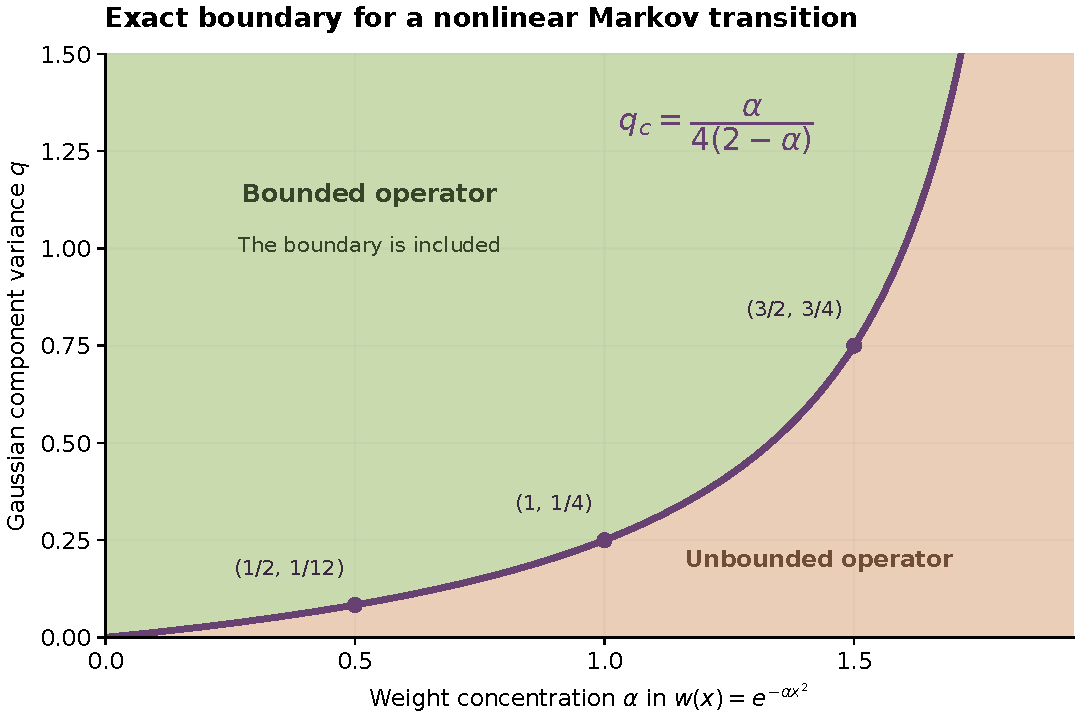
\includegraphics[width=.87\linewidth]{figures/phase-diagram.pdf}
\caption{Exact region for \eqref{eq:example}. The curve
$q=\alpha/[4(2-\alpha)]$ belongs to the bounded region.
The shaded regions are analytic classifications, not data
or estimates.}
\end{figure}}{}

\paragraph{An explicit obstruction below the boundary.}
Put $S=1+4q$, $c=S^{-1/2}$, $\vartheta=e^{-4/S}$,
$D=1-S^{-1}$, and $w=e^{\alpha y^2}$.
The ratio of the squared source representer norm for
$\operatorname{ev}_{iy}\circ T$ to the squared output
evaluation norm is exactly
\begin{equation}\label{eq:witness}
 c e^{-4Dy^2}
 \left[w^2+(1-w)^2+
             2w(1-w)\vartheta\cos(8y/S)\right].
\end{equation}
Since $\vartheta<1$, this grows exponentially in $y^2$
when $\alpha>2D$. Thus the failed cases have a direct
analytic witness, not only an existence argument.

\paragraph{Why individual kernel tests are insufficient.}
At $q=0,\alpha=1/2$, the operator is unbounded even though
it sends every real Gaussian section into $\HH_1$.
Its image is a finite sum of Gaussians with quadratic
exponents $1$ or $3/2$, and a Gaussian $e^{-\beta(x-c)^2}$
lies in $\HH_1$ exactly when $0<\beta<2$.
Checking the spanning sections one by one does not give a
uniform bound on their linear combinations.

\paragraph{Kernel width and gate width.}
For a general scalar width, $P=R=\sigma^2$ and $M=1$, one has
$D=4q/[\sigma^2(\sigma^2+4q)]$. A Gaussian-bump gate
$e^{-x^2/\ell^2}$ is then admissible exactly when
$\ell^2\ge\sigma^2(\sigma^2+4q)/(8q)$. A wider kernel requires a wider
gate: widening the test functions makes invariance harder, not easier.

\paragraph{Different component variances.}
The classification also applies directly to
\[
 X'\mid x\sim w_\alpha(x)N(x+1,1/4)
             +(1-w_\alpha(x))N(x-1,3/4).
\]
The two matrices of Theorem~\ref{thm:unequal} are the scalars
$D_+=1/2$ and $D_-=3/4$. Both weights have quadratic imaginary growth
rate $\alpha$, so this operator is bounded on $\HH_1$ exactly when
$0<\alpha\le1$. The component with the smaller variance supplies the
binding condition.

\paragraph{Contraction instead of noise.}
For $Q=0$, $M=a$ and $P=R=1$, the condition becomes
$\alpha\le2(1-a^2)$. For instance,
\[
 e^{-x^2}\delta_{x/2+1}
       +(1-e^{-x^2})\delta_{x/2-1}
\]
preserves $\HH_1$ and has nonlinear conditional mean
$x/2-1+2e^{-x^2}$. Thus state-dependent two-point noise
already supplies a valid nonlinear example.

\subsection{Probit and logistic gates}

Gating functions used in regime-switching and mixture-of-experts models
are usually probit or logistic. Theorem~\ref{thm:mixture} separates them
sharply. Write $\Phi$ for the standard normal distribution function and
$\sigma(w)=1/(1+e^{-w})$ for the logistic function.

\begin{corollary}[Gate classification]\label{cor:gates}
In the setting of Theorem~\ref{thm:mixture}, let $N=2$, let $M$ have
full column rank, and let $p_1(x)=\Psi(a^\top x+c)$, $p_2=1-p_1$, with
$a\in\R^d\setminus\{0\}$ and $c\in\R$.
\begin{enumerate}
\item If $\Psi=\Phi$, the operator is bounded if and only if
$aa^\top\preceq4D$.
\item If $\Psi=\sigma$, the operator is unbounded for every $P$, $R$, $M$,
$Q$ and pair of shifts.
\end{enumerate}
In the scalar setting of \eqref{eq:example}, a probit gate $\Phi(\beta
x)$ is admissible exactly when $\beta^2\le16q/(1+4q)$, while the
Gaussian-bump gate requires $\alpha\le8q/(1+4q)$.
\end{corollary}

\begin{proof}
(1) The entire extension of $\Phi$ is
$\Phi(w)=\tfrac12+(2\pi)^{-1/2}\int_0^we^{-t^2/2}\dd t$. Integrate
along $0\to iv\to u+iv$ for $w=u+iv$. The vertical part has modulus
$\int_0^{|v|}e^{s^2/2}\dd s\le\sqrt e+e^{v^2/2}$, by splitting at
$s=1$ and using $e^{s^2/2}\le se^{s^2/2}$ for $s\ge1$. The horizontal
part has modulus
$e^{v^2/2}\bigl|\int_0^ue^{-t^2/2}e^{-itv}\dd t\bigr|\le
\sqrt{\pi/2}\,e^{v^2/2}$. Hence $|\Phi(w)|\le C_0e^{(\im w)^2/2}$ with an
absolute constant $C_0$. At $z=x+iy$, $\im(a^\top z+c)=a\cdot y$, so
\[
 |p_1(z)|e^{-2y^\top Dy}\le C_0\exp\bigl(\tfrac12(a\cdot y)^2-2y^\top
 Dy\bigr).
\]
If $aa^\top\preceq4D$, then $D\succeq0$, the exponent is nonpositive,
and $|p_2|\le1+|p_1|$ gives the same bound for $p_2$; boundedness
follows from Theorem~\ref{thm:mixture}. Suppose instead that
$(a\cdot y_0)^2>4y_0^\top Dy_0$ for some $y_0$. If $a\cdot y_0=0$, then
$D$ has a negative direction and Theorem~\ref{thm:mixture} already gives
unboundedness, since its conditions imply $D\succeq0$. Otherwise choose real $x_0$ with
$a^\top x_0+c=0$ and put $z_s=x_0+isy_0$. Then $p_1(z_s)=\Phi(iv)$ with
$v=s\,a\cdot y_0$, and for $|v|\ge1$
\[
 |\Phi(iv)|\ge(2\pi)^{-1/2}\int_{|v|-1}^{|v|}e^{t^2/2}\dd t
 \ge(2\pi)^{-1/2}e^{(|v|-1)^2/2}.
\]
Hence $|p_1(z_s)|e^{-2s^2y_0^\top Dy_0}\to\infty$ as $s\to\infty$, and
Theorem~\ref{thm:mixture} gives unboundedness.

(2) Suppose $p_1$ agreed on $\R^d$ with an entire function $\tilde p$.
With $x_0$ as above and $e=a/|a|^2$, the entire function
$t\mapsto\tilde p(x_0+te)$ equals $\sigma(t)$ for real $t$, hence on the
connected set where the meromorphic function $\sigma$ is holomorphic.
But $\sigma$ has a pole at $t=i\pi$, so the entire function would be
unbounded near a finite point. This contradiction shows that $p_1$ has
no entire extension, and Theorem~\ref{thm:mixture} gives unboundedness.

In the scalar setting $D=4q/(1+4q)$, so $aa^\top\preceq4D$ reads
$\beta^2\le16q/(1+4q)$; the bump condition is
Corollary~\ref{cor:threshold}.
\end{proof}

The logistic gate fails for a structural reason, not a quantitative
one: any gate whose holomorphic extension has a singularity at a finite
point is excluded, however small the gate's slope. The probit gate is
excluded only above a slope threshold.

\paragraph{Continuous time.}
Whenever \eqref{eq:example} is bounded on $\HH_1$, it also
defines a bounded RKHS Markov semigroup
\[
 P_t=e^{t(T-I)}
     =e^{-t}\sum_{n=0}^{\infty}\frac{t^n}{n!}T^n .
\]
This is the jump process that waits an exponential time of rate one and
then moves according to \eqref{eq:example}. The series converges in
operator norm and $\norm{P_t}\le e^{t(\norm T-1)}$. This standard
uniformisation argument supplies nonlinear continuous-time examples with
a constant jump rate; state-dependent jump rates are not covered.

\section{Verification and remaining scope}\label{sec:verification}

This section states what the accompanying scripts check and which cases
the theorems leave open.

The theorems rest on the written proofs. The script
\texttt{code/verify.py} checks the Gaussian spectral constants, the tube
norm, the exact scalar thresholds, finite Gaussian Gram identities
against direct quadrature, the triangular-noise norms, the bandlimited
warping identity and the Gaussian smoothing formulas of
Appendix~\ref{app:spectrum} (97 checks). The script
\texttt{code/check\_extensions.py} checks, in 50-digit arithmetic, the
constants $c_*$, $t_*$ and $a_*$ of \eqref{eq:astar} and the claimed
norms for slopes $1$ to $4$; the growth bounds \eqref{eq:typetwo} for
the warping target and its dilations; the bound $|\Phi(w)|\le
C_0e^{(\im w)^2/2}$ on a grid and the divergence of the probit weight
ratio above the threshold; the unitary-conjugation form of the Fock
Gram matrix in Corollary~\ref{cor:fock} for random complex points in
two variables; and the scalar threshold identities of
Section~\ref{sec:example}. These finite calculations test constants and
implementations; they do not certify the analytic theorems. No
proof-assistant verification or external peer review has been
performed.

The mixture theorems are complete for finite mixtures with a common
linear part and fixed covariances. Mixtures whose branches have
different linear parts, state-dependent component covariances,
infinitely many state-dependent components, state-dependent L\'evy
kernels and general Markov transitions remain open. With different
linear parts the branch features can coincide at complex states, so the
uniform Gram bound of Lemma~\ref{lem:uniformgram} fails and a different
argument is needed. Quantitative approximation on compact sets is a
separate problem.

\appendix
\section{Exact smoothing norm and compactness}\label{app:spectrum}

This appendix records a classical Gaussian integral-operator
calculation (compare the parameter classification of Sang and Zhao
\cite{SangZhao2026}) in the normalisation of the nonlinear example. It
is a verification and interpretation tool, not an independent priority
claim.

On $\HH_1(\R)$ let $\mathcal S_qf(x)=\E f(x+N(0,q))$ and
$Y_{\alpha,q}=\Mult_{e^{-\alpha x^2}}\mathcal S_q$, where
$0<\alpha<2$. The multiplier calculation of Theorem~\ref{thm:mixture}
gives boundedness exactly for $q\ge q_c=\alpha/[4(2-\alpha)]$. For
necessity here, $\mathcal S_q$ maps $\HH_1$ onto its natural space
$\HH_{1+4q}$, up to a scalar isometry, as is immediate from its Fourier
multiplier. Thus boundedness of the product is equivalent to the
multiplier condition on that whole space.

\begin{proposition}\label{prop:spectrum}
At $q=q_c$, $Y_{\alpha,q}$ has norm one and is noncompact.
For $q>q_c$, put
\[
 \delta=q-q_c,\qquad
 u=\sqrt{\alpha(2-\alpha)\delta},\qquad
 \lambda=\sqrt{1+u^2}-u.
\]
Its singular values squared are $\lambda^{2n+1}$,
$n=0,1,\ldots$. Consequently
\begin{equation}\label{eq:HS}
 \norm{Y_{\alpha,q}}^2=\lambda,\qquad
 \norm{Y_{\alpha,q}}_{\rm HS}^2
   =\frac1{2u}
   =\frac1{\sqrt{\alpha(4q(2-\alpha)-\alpha)}}.
\end{equation}
\end{proposition}

\begin{proof}
Use the unitary Fourier transform. The map
$f\mapsto\pi^{-1/4}e^{\xi^2/8}\widehat f(\xi)$
is an isometry $\HH_1\to L^2(\R)$.
The conjugated operator has integral kernel
\begin{equation}\label{eq:gaussiankernel}
 K(\xi,\eta)=\frac1{2\sqrt{\pi\alpha}}
 \exp\!\left[-\frac{(\xi-\eta)^2}{4\alpha}
                  +\frac{\xi^2-\eta^2}{8}
                  -\frac{q\eta^2}{2}\right].
\end{equation}
At $q=q_c$ the exponent is $-a_0(\xi-s_0\eta)^2$,
where $a_0=(2-\alpha)/(8\alpha)$ and
$s_0=2/(2-\alpha)$. Thus the operator is a Gaussian
convolution followed by a unitary dilation. Its norm is
\[
 \frac1{2\sqrt{\pi\alpha s_0}}
        \int_{\R}e^{-a_0t^2}\dd t=1 .
 \]
A nonzero convolution operator on $L^2(\R)$ is noncompact,
as seen by translating a fixed input.

For $\delta>0$, integrating $K^*K$ in $\xi$ gives
\begin{equation}\label{eq:mehler}
 L(\eta,\zeta)=\sqrt{\frac{\beta}{\pi}}\,
 e^{-\beta(\eta-\zeta)^2-\delta(\eta^2+\zeta^2)/2},
 \qquad \beta=\frac1{4\alpha(2-\alpha)}.
\end{equation}
Write $v=\beta+\delta/2$ and
$\gamma=\sqrt{v^2-\beta^2}>0$.
The Gaussian $e^{-\gamma\eta^2}$ is an eigenfunction:
Gaussian integration gives eigenvalue
$\lambda_0=\sqrt{\beta/(v+\gamma)}$.
The Hermite generating function gives the complete eigenvalue
sequence
$\lambda_0[\beta/(v+\gamma)]^n$.
For clarity, this follows by integrating
$e^{-\gamma\zeta^2}
 \exp(2\sqrt{2\gamma}\,\zeta t-t^2)$ in
\eqref{eq:mehler}; completing the square replaces $t$
by $[\beta/(v+\gamma)]t$ and leaves the same Gaussian
Hermite generating function, multiplied by $\lambda_0$.
The Hermite functions form a complete orthogonal basis.
Since $\delta/(4\beta)=u^2$, algebra gives
$\lambda_0=\sqrt{1+u^2}-u=\lambda$.
The eigenvalues of $K^*K$ are therefore
$\lambda^{2n+1}$. Summing them proves \eqref{eq:HS}.
\end{proof}

For the Markov example, $T=L_-+
\Mult_{w_\alpha}(L_+-L_-)$, with $L_\pm f(x)=\mathcal S_qf(x\pm1)$.
If $q>q_c$, the second term is Hilbert--Schmidt, since
translations are unitary and \eqref{eq:HS} applies.
The mixture is then a compact perturbation of a
translation-invariant smoothing operator. This statement
does not make the whole Markov operator compact.

\section*{AI-use statement}
This manuscript was produced with AI assistance. The proofs were drafted
and checked with AI tools, and the computational checks were written and
run with them. Internal AI-assisted review was used; no external peer
review or formal proof verification has been carried out.

\begin{thebibliography}{99}
\bibitem{Evidence2026}
Anonymous. (2026).
\emph{When Gaussian kernel spaces are invariant under stochastic
dynamics: Transition rigidity, a Gaussian-component noise boundary
and a discontinuous diffusion limit} (Version 0.1.1-candidate).
Evidence Press.
\url{https://doi.org/10.5281/zenodo.24089772}

\bibitem{CCKT2026}
Cho, H. R., Choe, B. R., Koo, H., \& Tien, P. T. (2026).
\emph{The rigidity phenomenon for weighted composition operators on the
Fock spaces} (arXiv:2611.26206).
\url{https://arxiv.org/abs/2611.26206}

\bibitem{HaiHuyTien2026}
Hai, P. V., Huy, V. N., \& Tien, P. T. (2026).
\emph{Analytic tools and weighted composition operators on
Paley--Wiener spaces} (arXiv:2611.21261).
\url{https://arxiv.org/abs/2611.21261}

\bibitem{Hertel2026}
Hertel, M., Philipp, F. M., Schaller, M., \& Worthmann, K. (2026).
Koopman for stochastic dynamics: Error bounds for kernel extended
dynamic mode decomposition (kernel EDMD).
\emph{SIAM Journal on Applied Dynamical Systems, 25}(3), 2044--2083.
\url{https://doi.org/10.1137/26M1839689}

\bibitem{Ikeda2022}
Ikeda, M., Ishikawa, I., \& Sawano, Y. (2022).
Boundedness of composition operators on reproducing kernel
Hilbert spaces with analytic positive definite functions.
\emph{Journal of Mathematical Analysis and Applications, 511}(1), 126048.
\url{https://doi.org/10.1016/j.jmaa.2022.126048}
Preprint: arXiv:1911.11992.

\bibitem{Ishikawa2026}
Ishikawa, I. (2026).
\emph{Dynamical rigidity for weighted composition operators on
holomorphic function spaces} (arXiv:2604.03965).
\url{https://arxiv.org/abs/2604.03965}

\bibitem{Lebedev2012}
Lebedev, V. V. (2012).
On $L^2$-functions with bounded spectrum.
\emph{Sbornik: Mathematics, 203}(11), 1647--1653.
\url{https://doi.org/10.1070/SM2012v203n11ABEH004280}

\bibitem{LLYZ2026}
Lin, Z., Lu, Y., Yang, R., \& Zu, C. (2026).
\emph{Finite sums of weighted composition operators on the Fock space}
(arXiv:2611.19948).
\url{https://arxiv.org/abs/2611.19948}

\bibitem{Philipp2024}
Philipp, F. M., Schaller, M., Worthmann, K., Peitz, S., \&
N\"uske, F. (2024).
Error bounds for kernel-based approximations of the Koopman operator.
\emph{Applied and Computational Harmonic Analysis, 71}, 101657.
\url{https://doi.org/10.1016/j.acha.2024.101657}

\bibitem{Philipp2025}
Philipp, F. M., Schaller, M., Worthmann, K., Peitz, S., \&
N\"uske, F. (2025).
Invariance of Gaussian RKHSs under Koopman operators of stochastic
differential equations with constant matrix coefficients.
\emph{PAMM, 25}(1), e202400127.
\url{https://doi.org/10.1002/pamm.202400127}

\bibitem{SangZhao2026}
Sang, Y., \& Zhao, L. (2026).
\emph{Gaussian integral operator between Fock spaces}
(arXiv:2610.28279).
\url{https://arxiv.org/abs/2610.28279}

\bibitem{TienKhoi2019}
Tien, P. T., \& Khoi, L. H. (2019).
Differences of weighted composition operators between the Fock spaces.
\emph{Monatshefte f\"ur Mathematik, 188}(1), 183--193.
\url{https://doi.org/10.1007/s00605-018-1179-6}

\bibitem{TienKhoiFock2019}
Tien, P. T., \& Khoi, L. H. (2019).
Weighted composition operators between different Fock spaces.
\emph{Potential Analysis, 50}(2), 171--195.
\url{https://doi.org/10.1007/s11118-017-9678-y}

\bibitem{TienKhoi2020}
Tien, P. T., \& Khoi, L. H. (2020).
Weighted composition operators between Fock spaces in several variables.
\emph{Mathematische Nachrichten, 293}(6), 1200--1220.
\url{https://doi.org/10.1002/mana.201800197}
\end{thebibliography}
\end{document}
